\documentclass[border=7pt]{standalone}
\usepackage{tikz}
\usepackage{tkz-euclide}
\usepackage{amsmath}
\usepackage{amsfonts}
\usepackage{amssymb}

\newcommand\Mydiv[2]{%
$\strut#1$\kern.25em\smash{\raise.3ex\hbox{$\big)$}}$\mkern-8mu
        \overline{\enspace\strut#2}$}

\begin{document}
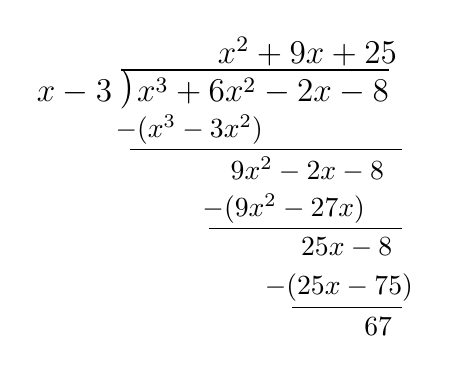
\begin{tikzpicture}
\node (c) at (-0.2,3) {\large \Mydiv{x-3}{x^3+6x^2-2x-8}};
\node (c) at (-0.5,2.5) {$-(x^3-3x^2)$};
\draw (-1.25, 2.25) -- (2.2,2.25);
\node (c) at (1,2) {$9x^2-2x -8$};
\node (c) at (0.7,1.5) {$-(9x^2-27x)$};
\draw (-.25, 1.25) -- (2.2,1.25);
\node (c) at (1.5,1) {$25x -8$};
\node (c) at (1.4,0.5) {$-(25x - 75)$};
\draw (0.8, .25) -- (2.2,.25);
\node (c) at (1.9,0) {$67$};
\node (c) at (1,3.5) {\large $x^2+9x+25$};



\end{tikzpicture}
\end{document}
